\documentclass[border=20pt]{standalone}
\usepackage{tikz}
\usetikzlibrary{
  positioning, 
  arrows.meta, 
  shapes, 
  shadows.blur,
  fit,
  backgrounds,
  calc
}
\usepackage{amsmath}
\usepackage{amssymb}

\begin{document}

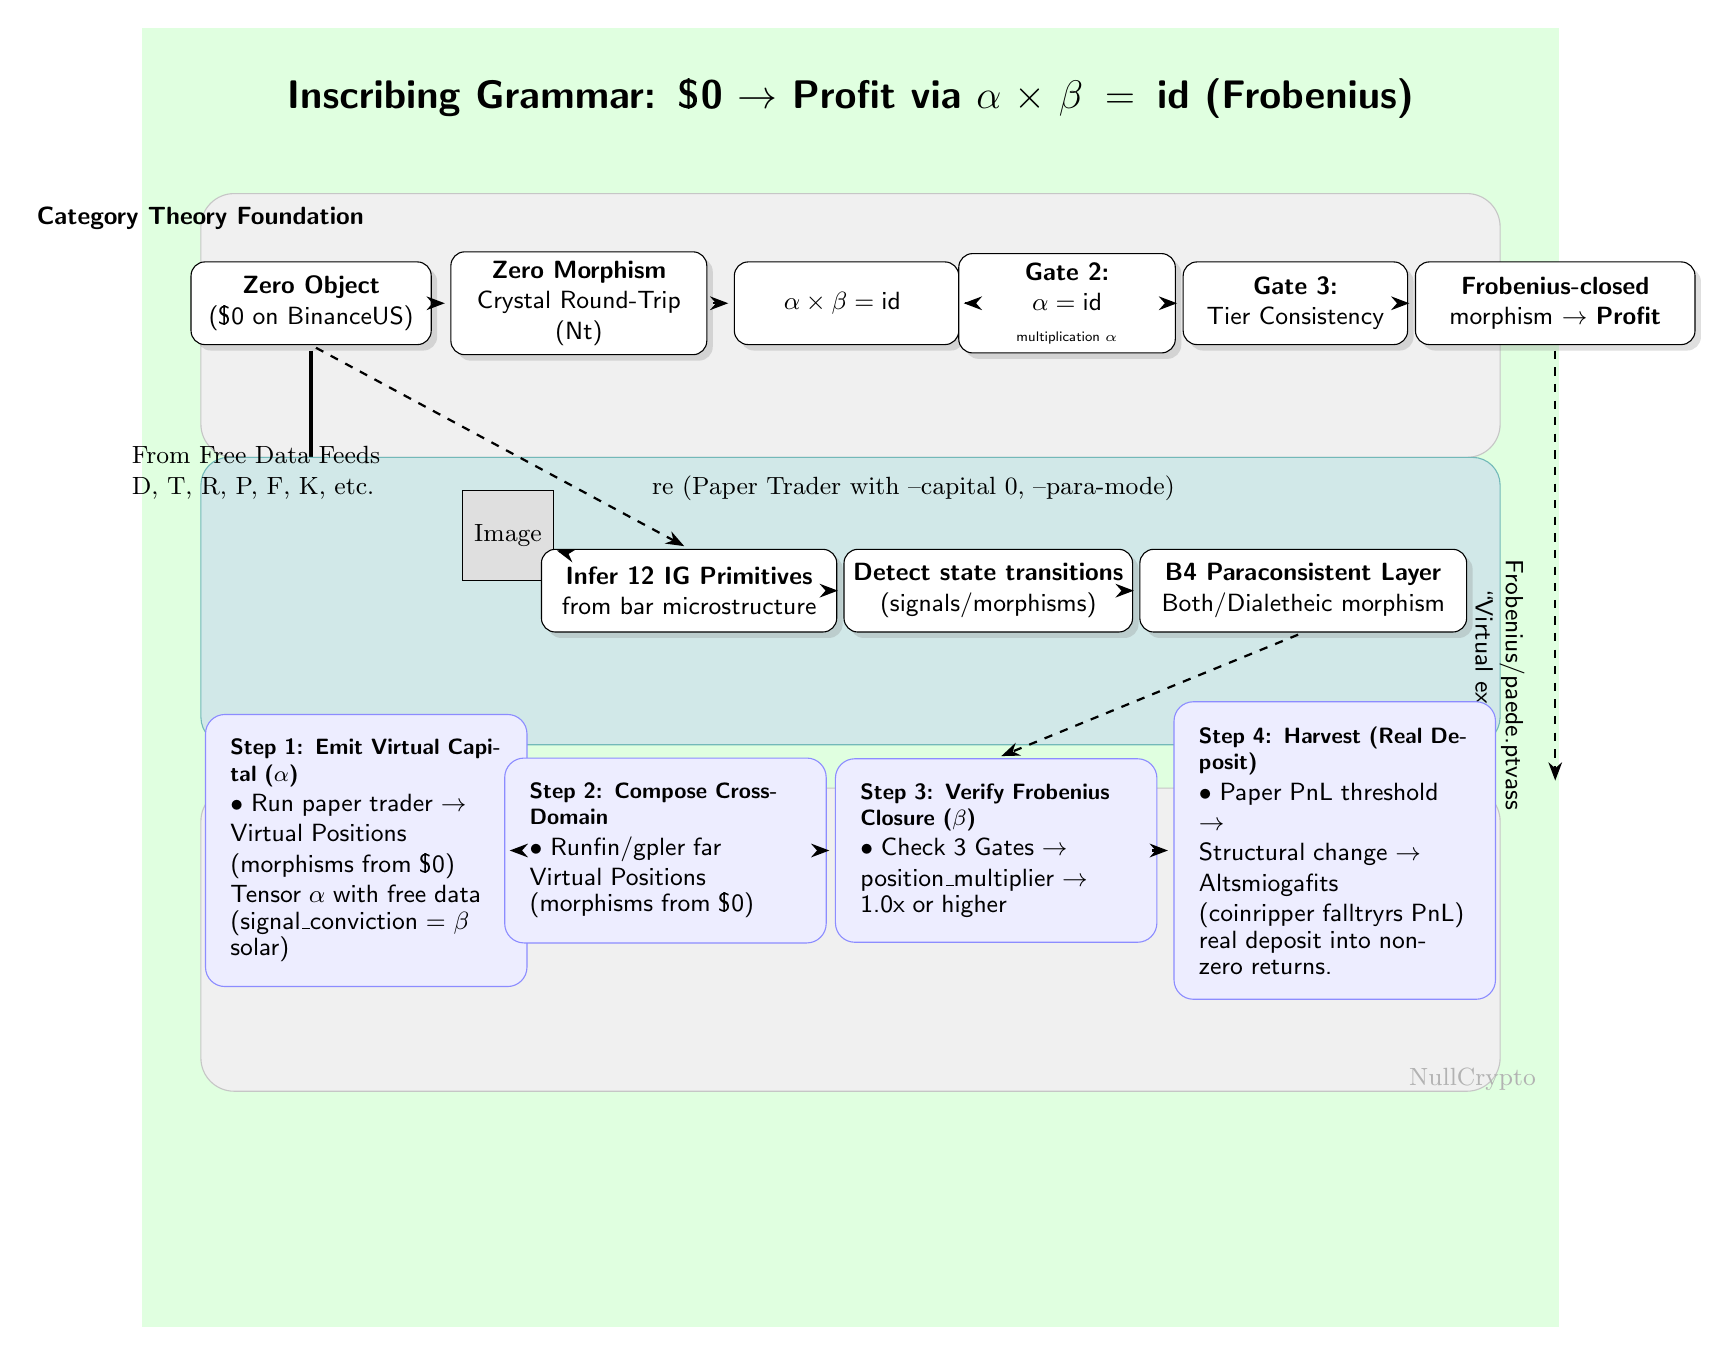
\begin{tikzpicture}[
  node distance=0.55cm and 1.05cm,
  box/.style={
    draw, 
    rounded corners=5pt, 
    minimum height=1.05cm, 
    align=center,
    font=\small\sffamily,
    fill=white,
    drop shadow={opacity=0.25}
  },
  section/.style={
    fill=gray!12,
    draw=gray!45,
    rounded corners=12pt,
    inner sep=14pt
  },
  midsec/.style={
    fill=teal!18,
    draw=teal!55,
    rounded corners=10pt,
    inner sep=12pt
  },
  stepbox/.style={
    fill=blue!7,
    draw=blue!45,
    rounded corners=7pt,
    inner sep=9pt,
    align=left,
    font=\footnotesize\sffamily,
    text width=3.45cm
  },
  arrow/.style={-{Stealth}, thick, shorten >=2pt, shorten <=2pt},
  title/.style={font=\Large\bfseries\sffamily, align=center}
]

% Background
\begin{scope}[on background layer]
  \fill[green!12] (-9,-8) rectangle (9,8.5);
\end{scope}

% TITLE
\node[title, text width=16.5cm] (title) at (0,7.6) {Inscribing Grammar: \$0 $\to$ Profit via $\alpha \times \beta = \text{id}$ (Frobenius)};

% ==================== CATEGORY THEORY FOUNDATION ====================
\node[section, minimum width=16.5cm, minimum height=3.35cm, anchor=north] (catsec) at (0,6.4) {};

\node[font=\bfseries\sffamily\small] at ([yshift=-9pt]catsec.north west) {Category Theory Foundation};

% Top row - tighter and better aligned
\node[box, minimum width=3.05cm] (zeroobj) at (-6.85,5) {
  \textbf{Zero Object} \\
  (\$0 on BinanceUS)
};

\node[box, minimum width=3.25cm] (zeromorph) at (-3.45,5) {
  \textbf{Zero Morphism} \\
  Crystal Round-Trip \\
  (Nt)
};

\node[box, minimum width=2.85cm] (eq) at (-0.05,5) {
  $\alpha \times \beta = \text{id}$
};

\node[box, minimum width=2.75cm] (gate2) at (2.75,5) {
  \textbf{Gate 2:} \\
  $\alpha = \text{id}$ \\
  \tiny multiplication $\alpha$
};

\node[box, minimum width=2.85cm] (gate3) at (5.65,5) {
  \textbf{Gate 3:} \\
  Tier Consistency
};

\node[box, minimum width=3.55cm] (profit) at (8.95,5) {
  \textbf{Frobenius-closed} \\
  morphism $\to$ \textbf{Profit}
};

% Top arrows
\draw[arrow] (zeroobj) -- (zeromorph);
\draw[arrow] (zeromorph) -- (eq);
\draw[arrow] (eq) -- (gate2);
\draw[arrow] (gate2) -- (gate3);
\draw[arrow] (gate3) -- (profit);

% Down from Zero Object
\draw[arrow, very thick] (zeroobj.south) -- ++(0,-1.85);

% ==================== MIDDLE SECTION ====================
\node[midsec, minimum width=16.5cm, minimum height=3.65cm, anchor=north] (midsec) at (0,3.05) {};

% Left data feeds
\node[align=left, font=\small] at (-7.55,2.85) {From Free Data Feeds \\ D, T, R, P, F, K, etc.};

% Image placeholder
\node[draw, minimum size=1.15cm, fill=gray!25, font=\small] (img) at (-4.35,2.05) {Image};

% Middle boxes - better spacing
\node[box, minimum width=3.75cm] (infer) at (-2.05,1.35) {
  \textbf{Infer 12 IG Primitives} \\
  from bar microstructure
};

\node[box, minimum width=3.65cm] (detect) at (1.75,1.35) {
  \textbf{Detect state transitions} \\
  (signals/morphisms)
};

\node[box, minimum width=4.15cm] (b4) at (5.75,1.35) {
  \textbf{B4 Paraconsistent Layer} \\
  Both/Dialetheic morphism
};

% Middle arrows
\draw[arrow] (img) -- (infer);
\draw[arrow] (infer) -- (detect);
\draw[arrow] (detect) -- (b4);

% Paper Trader label
\node[font=\small, align=center] at (0.8,2.65) {re (Paper Trader with --capital 0, --para-mode)};

% Right annotation
\node[rotate=270, font=\small\sffamily, align=center] at (8.25,0.15) {Frobenius/paede.ptvass \\ ``Virtual ex nihilo''};

% ==================== BOTTOM STEPS ====================
\node[section, minimum width=16.5cm, minimum height=3.85cm, anchor=north] (bottomsec) at (0,-1.15) {};

% Step 1
\node[stepbox] (s1) at (-6.15,-1.95) {
  \textbf{Step 1: Emit Virtual Capital ($\alpha$)} \\
  \small $\bullet$ Run paper trader $\to$ \\
  Virtual Positions \\
  (morphisms from \$0) \\
  Tensor $\alpha$ with free data \\
  (signal\_conviction = $\beta$ solar)
};

% Step 2
\node[stepbox] (s2) at (-2.35,-1.95) {
  \textbf{Step 2: Compose Cross-Domain} \\
  \small $\bullet$ Runfin/gpler far \\
  Virtual Positions \\
  (morphisms from \$0)
};

% Step 3
\node[stepbox] (s3) at (1.85,-1.95) {
  \textbf{Step 3: Verify Frobenius Closure ($\beta$)} \\
  \small $\bullet$ Check 3 Gates $\to$ \\
  position\_multiplier $\to$ \\
  1.0x or higher
};

% Step 4
\node[stepbox] (s4) at (6.15,-1.95) {
  \textbf{Step 4: Harvest (Real Deposit)} \\
  \small $\bullet$ Paper PnL threshold $\to$ \\
  Structural change $\to$ Altsmiogafits \\
  (coinripper falltryrs PnL) \\
  real deposit into non-zero returns.
};

% Step arrows
\draw[arrow] (s1) -- (s2);
\draw[arrow] (s2) -- (s3);
\draw[arrow] (s3) -- (s4);

% Cross connections
\draw[arrow, dashed, thick] (zeroobj.south) -- (infer.north);
\draw[arrow, dashed, thick] (b4.south) -- (s3.north);
\draw[arrow, dashed, thick] (profit.south) -- ++(0,-5.6);

% Null Crypto
\node[font=\small, color=gray!60] at (7.9,-4.85) {NullCrypto};

\end{tikzpicture}

\end{document}